\documentclass[margin,line]{resume}

\usepackage[latin1]{inputenc}
\usepackage[english,french]{babel}
\usepackage[T1]{fontenc}
\usepackage{fontawesome}
\usepackage{graphicx,wrapfig}
\usepackage{url}
\usepackage[colorlinks=true, pdfstartview=FitV, linkcolor=blue,
citecolor=blue, urlcolor=blue]{hyperref}
\pdfcompresslevel=9

\begin{document}
{\sc \Large Grishin Anton --- Junior developer \\}

\begin{resume}

  % === PICTURE ===

  \begin{wrapfigure}{R}{0.17\textwidth}
    \vspace{-0.9cm}
    \begin{center}
      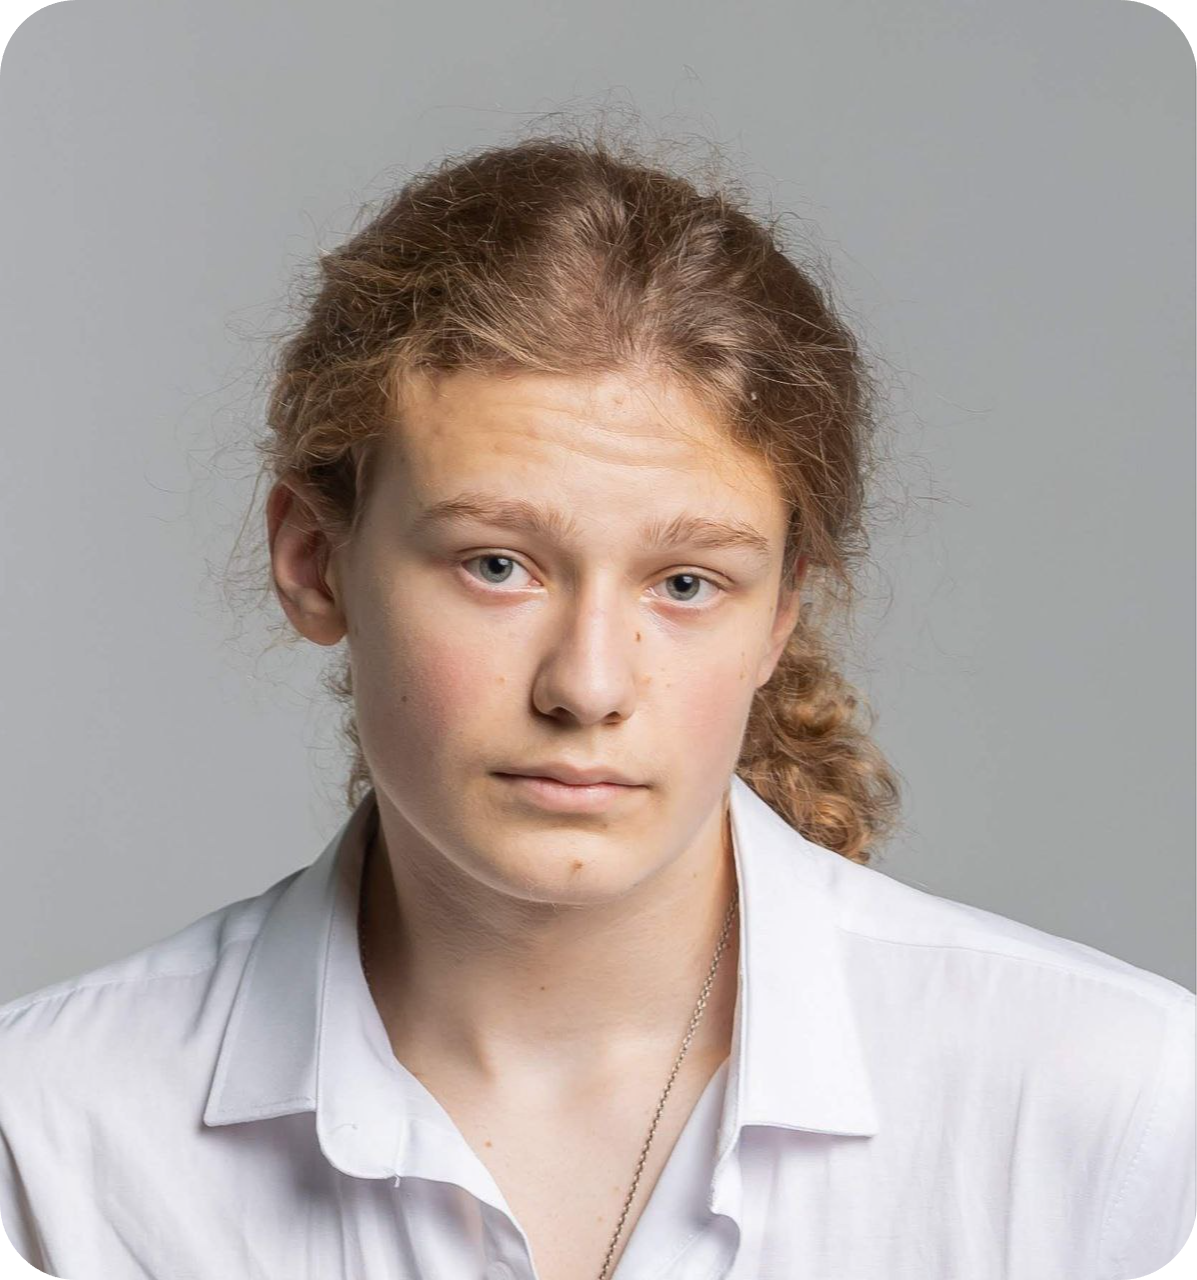
\includegraphics[width=0.17\textwidth]{avatar.png}
    \end{center}
    \vspace{-1cm}
  \end{wrapfigure}

  % === PERSONAL INFO ===

  \section{\mysidestyle Personal\\Information}
  Grishin Anton \\
  Moscow, Russia \\
  \faGithub  \space \href{https://github.com/alchemmist/}{@alchemmist} \\
  \faPaperPlane \space \href{https://t.me/alchemmist}{@alchemmist} \\
  \faLinkedin \space
  \href{https://www.linkedin.com/in/anton-grishin-6966a8362/}{anton-grishin} \\
  \faPhone \space +79150672638 \\
  \faEnvelope \space anton.ingrish@gmail.com \\

  % === OBJECTIVE ===

  \section{\mysidestyle About me}
  Improve the efficiency of the microwave and RF designers and
  structures. I focus on nonlinear devices at circuits level (such as
  HEMTs transistors) and at system level (HPA, Switches). That
  purpose requires an original use of an advanced RF instrumentation
  associated to a strong knowledge in terms of measured devices modeling.

  % === SKILLS ===

  \section{\mysidestyle Skills}\vspace{2mm}
  \begin{description}
    \item[Operating systems:] Unix, Linux and Windows
    \item[Programming languages:] Python, Go, JavaScript, WebTech (HTML, CSS).
    \item[Office softwares:] Latex, Microsoft Office, Libree Office.
    \item[Scientific softwares] Comsys, Maple, Matlab, Mathematica,
      Scilab, Keysight's VEE and ADS, NI LabVIEW.
    \item[Characterization tools:] Spectrum analyzers, scopes, AWG,
      VNA, LSNA, probe stations, high impedance probes. I have
      developed calibration procedures and automated calibration and
      measurements processes.
    \item[System Level Modeling:] Amplifiers, modulators and mixers
      with splines, neural networks or Volterra expansions. Bilateral
      Modeling by PhD model.
    \item[Circuit Level Modeling:] Linear, nonlinear and
      electrothermal models of HEMTs.
    \item[Languages:] French, English.
  \end{description}

  % === EDUCATION ===

  \section{\mysidestyle Education}
  Central University - Mathematics and Computer Science, 2028 \\

  % === CERTIFICATIONS ===

  \section{\mysidestyle Certifications}
  \textbf{National Instruments} Certified LabVIEW Associate Developer
  (CLAD) \hfill \textsl{July 2014-July 2016}\\

  % === AWARDS ===

  \section{\mysidestyle Awards}\vspace{4mm}
  \begin{list2}
  \item \textbf{Best Paper Award}, European Microwave Week - Galium
    Arsenide Application Symposium (GAAS), 2002 \\
    \textsl{\footnotesize{T. Reveyrand, C. Maziere, J.M. N\'ebus, R.
        Qu\'er\'e, A. Mallet, L. Lapierre, J. Sombrin, ``A calibrated
        time domain envelope measurement system for the behavioral
        modeling of power amplifiers'', European Microwave Week, GAAS
    2002, pp. 237-240, Milano, September 2002}}
    \vspace{1mm}
  \item \textbf{Best Student Paper Award}, Journ\'ees Nationales
    Micro-ondes (JNM), 2007 \\
    \textsl{\footnotesize{
        O. Jardel, F. De Groote, T. Reveyrand, C. Charbonniaud, J.P.
        Teyssier, R. Qu\'er\'e, D. Floriot, ``Mod\'elisation du drain-lag
        dans les mod\`eles \'electriques grand-signaux de transistors
        HEMTs AlGaN/GaN'', 15eme Journ\'ees Nationales Micro-ondes
    (JNM),3C1, Toulouse, Mai 2007.}}
  \end{list2}

  Up to 130 other refrences are available here : \\
  \vspace{-8mm}

  \href{http://www.microwave.fr/publications.html}{http://www.microwave.fr/publications.html}
  %\vspace{-1mm}

  % === INTERESTINGS ===
  \section{\mysidestyle Interestings}\vspace{2mm}
  \begin{description}
    \item[Philosophy] Unix, Linux and Windows
    \item[Books:] Unix, Linux and Windows
  \end{description}

  \vfill

  % === HISTORY ===

  \section{\mysidestyle History}\vspace{2mm}


  \begin{description}


    \item[Measurement Engineer (CNRS)]\small{XLIM \hfill \textsl{June
      2016-Present}}\\
    \item[Lecturer]\small{University of Colorado, Boulder \hfill
      \textsl{January 2016-May 2016}}\\
      ECEN 5014-003, ``Microwave Measurements and Calibration Fundamentals''
      \vspace{2mm}

    \item[Research Associate]\small{University of Colorado at Boulder
      \hfill \textsl{June 2013-May 2016}}\\
      Achievements:
      \begin{list2}
      \item{LabVIEW software for a ``Do-it-yourself'' Large-Signal
        Network Analyzer (LSNA)}
      \item{Time domain measurement setup in Scilab (VTD-SWAP)}
      \item{Outphasing PA characterizations}
      \item{Load-pull in time-domain}
      \end{list2}
      \vspace{2mm}


    \item[Measurement Engineer (CNRS)]\small{XLIM \hfill
      \textsl{December 2007-May 2013}}\\
      Achievements:
      \begin{list2}
      \item{Korrigan European Project activities (RTP
            N$^{\circ}$102.052 funded within the EUROPA framework in the
          CEPA2 priority area - ends early 2009) : GaN HEMTs circuits
          level modeling from european foundries (Thales / QinetiQ) for
        HPA, LNA and Switches}
      \item{Time domain measurement setup (LSNA) development on
        Scilab-TCL/TK (GUI, calibration and measurement automation)}
      \item{Development of HEMTs modeling tools (Scilab)}
      \item{Contractual measurements such as load-pull, linearity,
        high impedance probe in both frequency (VNA) and time domain (LSNA)}
      \end{list2}
      \vspace{2mm}


    \item[Research Associate - Visiting Scholar]\small{University of
      Colorado at Boulder \hfill \textsl{February 2012-July 2012}}\\
      GaN HEMTs based rectifiers characterizations and analysis
      \vspace{2mm}

    \item[Research Engineer (CNRS)]\small{XLIM \hfill \textsl{May
      2005-November 2007}}\\
      Achievements:
      \begin{list2}
      \item{Frequency domain load-pull measurement setup (VNA in
          receiver mode with pulse capabilities) developpemnt with
          Scilab (calibration procedures, measurement automation, data
        processing)}
      \item{Large signal caracterization of transistor (mainly
          european GaN in the framework of Korrigan}
        \item{Korrigan WP3.3 workpackage leader in Korrigan.
            Developpement of a internet database (Php / mySQL) to let
          partners share data and informations}
        \item{GaN HEMTs ``spice-like'' nonlinear models}
        \end{list2}
        \vspace{2mm}


      \item[Research Engineer]\small{NMDG Engineering bvba \hfill
        \textsl{November 2004-February 2005}}\\
        Implementation of the High Impedance Probe module
        (calibration and measurements) in the commercial LSNA
        Software (based on Mathematica)

        \vspace{2mm}


      \item[Postdoctoral scientist]\small{CNES (French Space Agency)
        \hfill \textsl{October 2003-September 2004}}\\
        Development of characterization tools interfaces within the
        free open-source scientific package Scilab

        \vspace{2mm}


      \item[Postdoctoral scientist]\small{CNES (French Space Agency)
        \hfill \textsl{October 2002-September 2003}}\\
        Achievements:
        \begin{list2}
        \item{Large Signal Network Analysis (LSNA) characterizations
          in time-domain}
        \item{Development of a new LSNA module in order to
            investigate time domain waveforms at internal nodes of
            MMICs with high impedance probes (HIP) to validate circuits
          designs and to analyze nonlinear parametric stability}
        \item{Large Signal Network Analysis (LSNA) characterizations
          in time-domain}
        \end{list2}
        \vspace{2mm}


      \item[Researcher]\small{IRCOM / University of Limoges \hfill
        \textsl{October 1998-September 2002}}\\
        Achievements:
        \begin{list2}
        \item{Development of the RF time-domain envelope measurement
          setup (hardware and software)}
        \item{Development of the calibration procedure of the
          time-domain envelope measurement setup}
        \item{Power amplifiers characterizations : Load-pull, IM3, NPR}
        \item{Behavioral modeling of nonlinear devices with memory
          effects for system level}
        \item{Development of a dynamic complex gain model with neural networks}
        \end{list2}
        \vspace{2mm}


      \item[Lecturer]\small{University of Limoges \hfill
        \textsl{October 1998-September 2002}}\\
        RF devices, analog/digital communication systems, signal
        processing, propagation waves...
        \vspace{2mm}


      \item[Postgraduate student]\small{IRCOM / University of Limoges
        \hfill \textsl{February 1998-July 1998}}\\
        Circuits level simulations of IM3 and NPR in order to
        optimize the trade-off between linearity and efficiency

    \end{description}


  \end{resume}
  \end{document}
